\section{Theorie}
\label{sec:Theorie}

In diesem Versuch wird die Funktionsweise eines Reinst-Germanium-Detektors diskutiert
und verschiedene Proben anhand aufgenommener Spektren charakterisiert.
Dazu werden im Folgenden die verschiedenen Mechanismen zur Energiedeposition von
$\gamma$-Strahlung in Materie erläutert, der Aufbau eines Halbleiter-Detektors
dargestellt und ein typisches Spektrum einer monochromatischen $\gamma$-Quelle diskutiert.

Der Intensitätsverlust eines $\gamma$-Strahls in Materie ist abhängig von
der Schichtdicke des Materials, der Elektronendichte $n$ und dem
Wirkungsquerschnitt $\sigma$.
Letzterer ist durch eine den Elektronen zugeordnete Fläche motiviert.
Diese Fläche lässt sich dann auf eine Wahrscheinlichkeit $W$ umrechnen,
mit welcher die Wechselwirkung eintritt. Für eine infinitesimale Schichtdicke
$\symup{d}x$ mit Gesamtfläche $F$ ergibt sich
\begin{equation*}
	\symup{d}W = \frac{n\:F\:\symup{d}x\:\sigma}{F} = n\:\sigma\:\symup{d}x
\end{equation*}
und nach Integration
\begin{equation}
	N\left(D\right) = N_\text{0} \cdot \exp^{-n\:\sigma\:D}
	\label{eqn:Intensitaet-Exp}
\end{equation}
mit der Schichtdicke $D$ und Anfangsintensität $N_\text{0}$.
Die Größe $\mu = n\:\sigma$ wird Extinktionskoeffizient genannt.
Eine weitere wichtige Größe ist die Aktivität $A$ eines $\gamma$-Strahlers,
welche die Anzahl der Zerfälle oder Emissionen pro Zeit.
Sie ist gegeben durch
\begin{equation}
	A\left(t\right) = A_0 \cdot \exp\left(-\frac{\ln 2}{T_{\sfrac{1}{2}}} t\right)
	\label{eqn:AktivitaetFormel}
\end{equation}
mit der Halbwertszeit $T_{\sfrac{1}{2}}$ und Anfangsintensität $A_0$.
Im Anschluss sind die Prinzipien und Wirkungsquerschnitte von drei
Wechselwirkungen näher betrachtet.

\subsection{Photo-Effekt}
\label{sec:Photo-Effekt}

Beim Photo-Effekt wechselwirkt ein $\gamma$-Quant mit einem Hüllenelektron. Dabei
wird das Quant absorbiert und das Elektron verlässt die Atomhülle.
Hierzu muss die Energie des Quants also mindestens die Bindungsenergie des
Elektrons betragen.
Der nun unbesetzte Zustand in der Atomhülle wird durch ein Elektron aus
einem höheren Orbital besetzt, das dabei ein $\gamma$-Quant mit charakteristischer
Energie emittiert. Die Lücke in dem höheren Orbital wird dann wiederum durch
ein Elektron aus einem noch höheren Orbital aufgefüllt und so weiter.

Der Wirkungsquerschnitt des Photo-Effekts ist abhängig von der Energie der
$\gamma$-Quanten und der Kernladungszahl $Z$.
Bei natürlichen Strahlern ergibt sich eine Abhängigkeit von
\begin{equation*}
	\sigma_\text{Ph} \sim Z^\alpha E^\delta
\end{equation*}
mit $4 < \alpha < 5$ und $\delta \approx \num{-3.5}$.
Für niedrige $\gamma$-Energien sind zudem Unstetigkeiten im Wirkungsquerschnitt
erkennbar, wenn die Energie genau der Bindungsenergie einer Schale entspricht.

\subsection{Compton-Effekt}
\label{sec:Compton-Effekt}

Im Korpuskelmodell des Lichts kann der Compton-Effekt als unelastische
Streuung an einem Elektron aufgefasst werden.
Unter der Annahme eines ruhenden Elektrons lässt sich mit Hilfe von Impuls-
und Energieerhaltung die Energie des gestreuten $\gamma$-Quants zu
\begin{equation}
	E_{\gamma'} = E_\gamma
	\frac{1}{1 + \varepsilon \left(1 - \cos \psi_\gamma\right)}
	\label{eqn:Compton-Energy}
\end{equation}
mit der Abkürzung
\begin{equation*}
	\varepsilon \equiv \frac{E_\gamma}{m_\text{0}\:c^2}
\end{equation*}
berechnen.
Hierbei bezeichnet $m_0$ die Ruheenergie des Elektrons und
$c$ die Lichtgeschwindigkeit im Vakuum.
Bei einem Streuwinkel von \SI{180}{\degree} ist der Energieübertrag
\begin{equation*}
	E_\text{l,max} = E_\gamma \frac{2 \varepsilon}{1 + 2 \varepsilon} < E_\gamma
\end{equation*}
an das Elektron maximal.
Im Unterschied zum Photo-Effekt wird nur ein Teil der $\gamma$-Energie übertragen,
sodass nicht die gesamte Energie des $\gamma$-Quants im Detektor deponiert werden kann und
das Quant den Detektor nach dem Compton-Effekt wieder verlassen kann.
Der im Detektor deponierte variable Anteil der $\gamma$-Energie lässt keine
Bestimmung dieser zu, sodass der Compton-Effekt im Detektor einen Störfaktor
darstellt.

Von Interesse ist der differentielle Wirkungsquerschnitt nach der Energie der
Elektronen, da nur diese an den Detektor abgegeben wird. Hierzu
wird der Wirkungsquerschnitt für $\varepsilon \rightarrow 0$ betrachtet,
welcher durch
\begin{equation*}
	\sigma_\text{Compton} = \frac{3}{4} \sigma_\text{Th}
	= \frac{3}{4} \cdot \frac{8}{3} \pi
	\left(\frac{e_0}{4\:\pi\:\varepsilon_0\:c^2\:m_0}\right)^2
\end{equation*}
mit dem Thomsonschen Wirkungsquerschnitt $\sigma_\text{Th}$ und der Elementarladung $e_0$ gegeben ist.
Hierbei wurde angenommen, dass sich die Elektronen bei Anregung durch die
$\gamma$-Quanten wie Hertzsche Dipole verhalten.
Wird dieser Ausdruck nach der Energie abgeleitet, ergibt sich
\begin{equation}
	\frac{\symup{d}\sigma}{\symup{d}E} =
	\frac{3}{8} \sigma_\text{Th} \frac{1}{m_0\:c^2\:\varepsilon^2}
  B
	\left\{2 + \left(\frac{E}{h \nu - E}\right)^2
	\left(\frac{1}{\varepsilon^2} + \frac{h \nu - E}{h \nu} - \frac{2}{\varepsilon}
	\left(\frac{h \nu - E}{h \nu}\right)\right)\right\}
	\label{eqn:Compton-Wirkungsquerschnitt}
\end{equation}
mit dem Planck'schen Wirkungsquantum $h$ und der Frequenz des $\gamma$-Quants $\nu$.
Der Verlauf dieses Wirkungsquerschnitts ist beispielhaft in Abbildung \ref{fig:Compton-Wirkungsquerschnitt}
dargestellt. Die sogenannte Compton-Kante kennzeichnet den maximalen Energieübertrag
$E_\text{l,max}$.

\begin{figure}
	\centering
	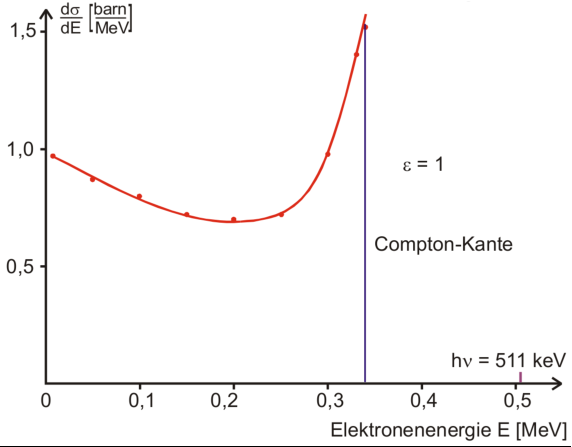
\includegraphics[height=7.0cm]{images/Compton-Wirkungsquerschnitt.pdf}
	\caption{Der differentielle Wirkungsquerschnitt nach \eqref{eqn:Compton-Wirkungsquerschnitt}
	in Abhängigkeit von der Elektronenenergie \cite[7]{anleitung}.}
	\label{fig:Compton-Wirkungsquerschnitt}
\end{figure}
\FloatBarrier

\subsection{Paarerzeugung}
\label{sec:Paarerzeugung}

Bei $\gamma$-Energien größer als $2 m_0 c^2$ ist ein Umwandlung des $\gamma$-Quants in ein
Elektron und ein Positron möglich.
Hierzu muss aus Impulserhaltungsgründen ein Stoßpartner in Form eines Hüllenelektrons
oder Atoms vorhanden sein.
Aufgrund der geringen Masse des Elektrons ist dessen Rückstoßenergie
bei der Paarerzeugung groß, sodass die Schwellwertenergie $4 m_0 c^2$ beträgt.
Einen möglichen Effekt nach der Paarerzeugung stellt die Rekombination des Positrons
mit einem weiteren Elektron dar. Die zwei daraus entstehenden $\gamma$-Quanten können
ihre gesamte Energie, oder auch nur einen Teil ihrer Energie im Detektor deponieren.
% TODO: Was bedeutet SEP/DEP?
Weiterhin können Elektron und Positron Energie in Form von Bremsstrahlung verlieren, die dann
den Detektor verlässt.
Die Energie des $\gamma$-Quants würde folglich zu gering rekonstruiert.

Bei der Berechnung des Wirkungsquerschnitts der Paarerzeugung ist die Position des Stoßpartners
von Bedeutung, da sich das Coulombfeld des Kerns mit größerem Abstand verändert.
Hüllenelektronen in niedrigen Schalen schirmen das Coulombfeld ab, sodass die
Angabe des Wirkungsquerschnitts auf zwei Grenzfälle beschränkt ist.
Bei Paarbildung in Kernnähe ist kaum Abschirmung durch Hüllenelektronen vorhanden
und es ergibt sich
\begin{equation*}
	\sigma_\text{Pa} = \alpha\:r_\text{e}^2\:Z^2
	\left(\frac{28}{9} \ln2\varepsilon - \frac{218}{27}\right)
\end{equation*}
mit der Sommerfeldschen Feinstrukturkonstanten $\alpha$.
Diese Gleichung ist jedoch nur für $10 < E_\gamma < \SI{25}{\mega\electronvolt}$ gültig.
Außerhalb der Elektronenhülle wird das Kernfeld stark abgeschirmt und es gilt
\begin{equation*}
	\sigma_\text{Pa} = \alpha\:r_\text{e}^2\:Z^2
	\left(\frac{28}{9} \ln\frac{183}{\sqrt[\leftroot{-1}\uproot{2}\scriptstyle 3]Z} - \frac{2}{27}\right)
\end{equation*}
für $\gamma$-Energien größer \SI{500}{\mega\electronvolt}.

\begin{figure}
	\centering
	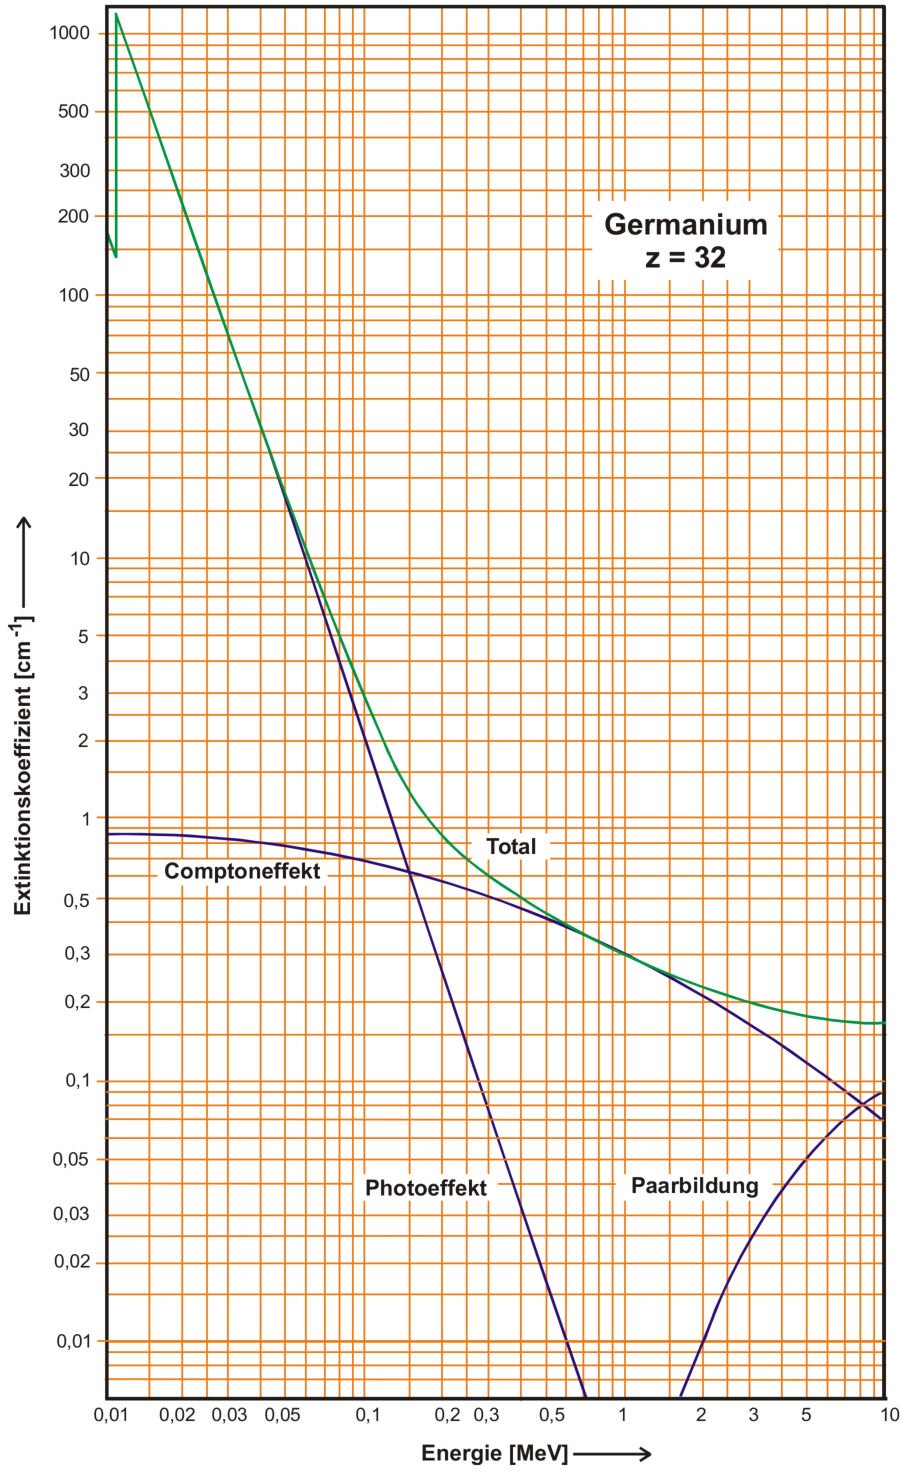
\includegraphics[width=.9\textwidth]{images/Wirkungsquerschnitte-gesamt.pdf}
	\caption{Extinktionskoeffizienten des Photoeffekts, Comptoneffekts und der Paarbildung \cite[9]{anleitung}.}
	\label{fig:Wirkungsquerschnitte-gesamt}
\end{figure}
Abschließend sind in Abbildung \ref{fig:Wirkungsquerschnitte-gesamt} die Extinktionskoeffizienten
der drei erläuterten Effekte aufgetragen. Es zeigt sich, dass für kleine Energien der Photoeffekt
dominant ist, während für hohe Energien die Paarbildung einsetzt.
Weiterhin ist bei ungefähr \SI{0.01}{\mega\electronvolt} eine Unstetigkeit im Koeffizienten des
Photoeffekts dargestellt, wenn die $\gamma$-Energie genau der Übergangsenergie zweier
Energieniveaus entspricht.

\subsection{Funktionsweise eines Halbleiter-Detektors}
\label{sec:HLDetektor}

Halbleiter-Detektoren ermöglichen eine hohe Energieauflösung bei der Untersuchung von $\gamma$-Strahlung.
Die Hauptkomponente bildet dabei eine Halbleiterdiode, welche aus zwei angrenzenden \ce{Ge}-Bereichen
besteht, die unterschiedlich dotiert sind.
An der Grenzfläche bildet sich durch Rekombination eine ladungsträgerarme Zone aus.
Fallen $\gamma$-Quanten in diese Zone, heben sie bei einer $\gamma$-Energie oberhalb
der Bandlücke ein Elektron in das Leitungsband.
Das Elektron erfährt wiederum eine Kraft in Richtung der p-dotierten
Seite der Diode und regt auf dem Weg dorthin weitere Elektronen an.
Ebenso bewegen sich die so entstandenen Löcher in Richtung der n-dotierten Schicht. Ist die
Diode an einen Strommesser angeschlossen, so lässt sich bei Einfall eines $\gamma$-Quants ein
Strompuls messen, dessen Höhe proportional zur im Detektor deponierten Energie ist.
Außerhalb der Verarmungszone ist das Feld zwischen den Bereichen zu klein, um das erzeugte Elektron-Loch-Paar
zu trennen, bevor es wieder rekombiniert.

Um den Potentialsprung $U_\text{D}$ und damit die Breite der Verarmungszone zu vergrößern,
wird eine äußere Spannung $U$ angelegt.
Dies ist in Abbildung \ref{fig:SchematischerPotentialverlauf} dargestellt.
Thermisch angeregte Ladungsträger aus Restverunreinigungen im Kristall verschlechtern
jedoch die Detektionseigenschaften.
Um den so entstehenden Blindstrom möglichst gering zu halten wird der
Detektor üblicherweise mit siedendem Stickstoff auf ungefähr \SI{77}{\kelvin} gekühlt.
Weiterhin wird die Dotierung so gewählt, dass die Breite $d$ der Verarmungszone möglichst groß ist.
Für eine deutlich höhere Elektronendichte der n-dotierten Donatorschicht $n_\text{D}$ im
Vergleich zur p-dotierten Akzeptorschicht $n_\text{A}$ ergibt sich näherungsweise
\begin{equation}
	d \approx \sqrt{\frac{2\:\varepsilon\:\varepsilon_0}{e_0} \left(U_\text{D} + U\right) \frac{1}{n_\text{A}}}
	\label{eqn:BreiteVerarmungszone}
\end{equation}
mit der Permittivität des Vakuums $\varepsilon_0$ und der Permittivität von Germanium $\varepsilon$.
Es zeigt sich, dass für eine möglichst geringe Elektronendichte der Akzeptorschicht und hohe
Sperrspannungen die Verarmungszone von einigen \si{\micro\meter} auf \SI{3}{\centi\meter} vergrößert werden kann.
\begin{figure}
	\centering
	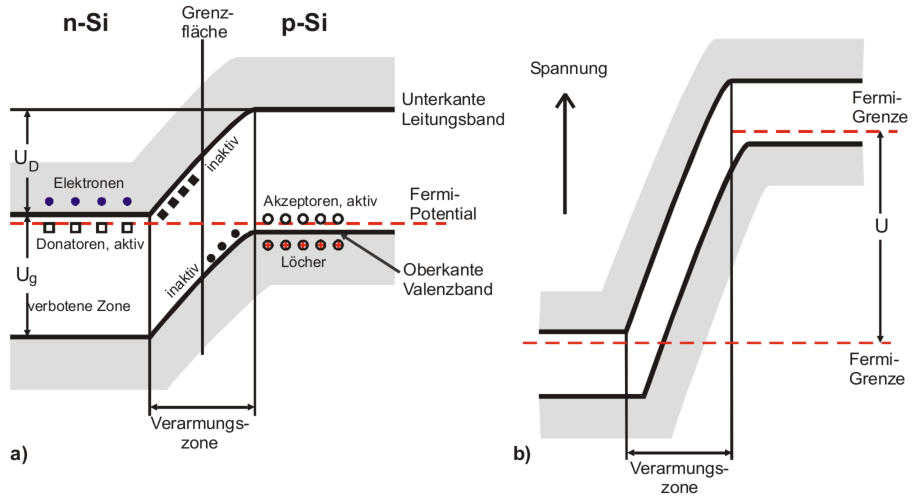
\includegraphics[width=\textwidth]{images/Schematischer-Potentialverlauf.pdf}
	\caption{Schematischer Potentialverlauf an der Grenzfläche zwischen n- und p-dotiertem
	Silizium a) ohne und b) mit angelegter externer Spannung am Beispiel \ce{Si}~\cite[12]{anleitung}.}
	\label{fig:SchematischerPotentialverlauf}
\end{figure}

\subsection{Kenngrößen eines Halbleiter-Detektors}
\label{sec:KenngroessenHLDetektor}

Um zwei Spektrallinien $E_1$ und $E_2$ voneinander unterscheiden zu können, müssen
sich die Mittelwerte mindestens um die Halbwertsbreite $\increment E_{\sfrac{1}{2}}$
der Impulshöhenverteilung des Detektors bei $\gamma$-Strahlung unterscheiden.
Diese Halbwertsbreite ist von der Anzahl der bei Absorption eines $\gamma$-Quants
freigesetzten Elektron-Loch-Paare $n$ festgelegt.
Für die benötigte Energie zur Bildung eines Elektron-Loch-Paares wurde im Mittel
$E_\text{EL} = \SI{2.9}{\electronvolt}$ bei \SI{77}{\kelvin} gemessen,
obwohl die Bandlücke zwischen Valenz- und Leitungsband lediglich
$E_\text{B} = \SI{0.67}{\electronvolt}$ beträgt.
Folglich muss bei der Bestimmung der Standardabweichung $\sigma$ der Verteilung von $n$ berücksichtigt werden, dass die
Erzeugung der Elektron-Loch-Paare nur unter Beteiligung von Phononen statt findet.
Die $\gamma$-Anregungsenergie verteilt sich statistisch auf das Elektron und Phononen.
Somit wird ein Teil der Fluktuationen der Ladungsträgererzeugung durch Fluktuationen der
Phononenanregung kompensiert und es ergibt sich
\begin{equation}
	\sigma = \sqrt{F\:\mean{n}}
\end{equation}
mit dem sogenannten Fano-Faktor $F$ und dem Mittelwert der Verteilung $\mean{n}$.
Da $n >> 1$ geht die Poissonverteilung in eine Gaußverteilung über und es ergibt sich
\begin{equation}
	\increment E_{\sfrac{1}{2}} = \sqrt{8 \ln2} \frac{\sigma}{\mean{n}} E_\gamma
  \sim \sqrt{E_\text{EL}}
\end{equation}
und bei einer typischen $\gamma$-Energie von \SI{500}{\kilo\electronvolt} eine
Halbwertsbreite von $\sim \SI{895}{\electronvolt}$.
Diese ist im Vergleich zu anderen auf dem Ionisationsprizip beruhenden
Detektorarten sehr gering.
Beispielhaft beträgt $E_\text{EL}$ für Proportionalzählrohre
\SIrange[range-phrase=\text{ bis }]{20}{30}{\electronvolt} und für Szintillationszähler
\SIrange[range-phrase=\text{ bis }]{500}{600}{\electronvolt} bei $F = \num{1}$.

Die Energieauflösung des Detektors wird durch weitere Effekte beschränkt, die praktisch unkorrelliert sind.
Ein Effekt ist das Rauschen aufgrund eines in Abschnitt \ref{sec:HLDetektor} erklärten Leckstroms
durch thermische Elektronen, welcher in einer zusätzlichen Halbwertsbreite $H_\text{R}$ der Energieverteilungskurve resultiert.
Dieser kann durch Abkühlung des Detektors reduziert werden.
Weiterhin existieren Feldinhomogenitäten aufgrund des Aufbaus des Detektors ($H_\text{I}$), die jedoch
mit steigender angelegter Spannung kleiner werden.
Schließlich spielt auch das Rauschen des Signalverstärkers ($H_\text{E}$) eine Rolle. Dieses Rauschen
kann durch Kühlung der ersten Verstärkerstufe reduziert werden.
Die Halbwertsbreite unter Berücksichtigung aller Störeffekte $H_\text{ges}$
ist schließlich durch
\begin{equation}
  H_\text{ges}^2 = \increment E_{\sfrac{1}{2}}^2 + H_\text{R}^2
  + H_\text{I}^2 + H_\text{E}^2
\end{equation}
gegeben.

Zur Bestimmung der Aktivität einer Probe $A$ spielt eine weitere Kenngröße des Detektors eine
Rolle, die sogenannte Vollenergie-Nachweiseffizienz $Q$.
Sie gibt die Effizienz an, mit welcher Wahrscheinlichkeit das Quant mit dem Detektor
wechselwirkt und dabei die gesamte Energie deponiert.
Das gemessene Zählergebnis einer $\gamma$-Linie $Z$ ist gegeben durch
\begin{equation}
	Z = \frac{\Omega}{4\:\pi} A\:W\:Q
	\label{eqn:Vollenergie-Nachweiseffizienz}
\end{equation}
mit der Emissionswahrscheinlichkeit der bestimmten Linie $W$
und dem Raumwinkel $\Omega$, den der Detektor aus Sicht des Strahlers einnimmt.

\subsection{Spektrum einer monochromatischen Gamma-Quelle}
\label{sec:TypischeQuelle}

Das Spektrum einer monochromatischen $\gamma$-Quelle ist in Abbildung \ref{fig:typisches-Spektrum}
dargestellt. Aufgetragen ist die Kanalfüllung gegen die Energie der $\gamma$-Quanten.
Aufgrund der Aluminium-Abschirmung des \ce{Ge}-Detektors nach Abschnitt \ref{sec:AufbauDetektor} existiert eine
minimale detektierbare Energie der $\gamma$-Quanten, die als Empfindlichkeitsgrenze eingezeichnet ist.
Der Vollenergiepeak entsteht, wenn das einfallende $\gamma$-Quant seine gesamt Energie im Detektor
deponiert. Es wird also nach möglichen Compton-Streuungen Photo-absorbiert
oder es tritt direkt der Photoeffekt auf.
Bei Energien unterhalb des Vollenergiepeaks ist das sogenannte Compton-Kontinuum beobachtbar. Je nach
Energieübertrag des $\gamma$-Quants auf das Elektron wird unterschiedlich viel Energie im Detektor deponiert,
bis zu einem maximalen Energieübertrag an der Compton-Kante.
Weiterhin ist ein Rückstreupeak aufgetragen, welcher dadurch entsteht, dass die $\gamma$-Quanten erst
nach einer Compton-Streuung in den Detektor gelangen.
Hierbei treten große Streuwinkel auf, sodas sich die Position des Rückstreupeaks im
Spektrums durch Einsetzen eines Winkels von \SI{180}{\degree} in Formel
\eqref{eqn:Compton-Energy} zu
\begin{equation}
  E_{\gamma'} = E_\gamma \frac{\varepsilon}{1 + 2 \varepsilon}
\end{equation}
abgeschätzt werden kann.
Oberhalb der Compton-Kante ist ebenfalls eine Kanalfüllung beobachtbar. Diese lässt sich mit mehrfachen
Compton-Streuungen eines Photons erklären.

\begin{figure}
	\centering
	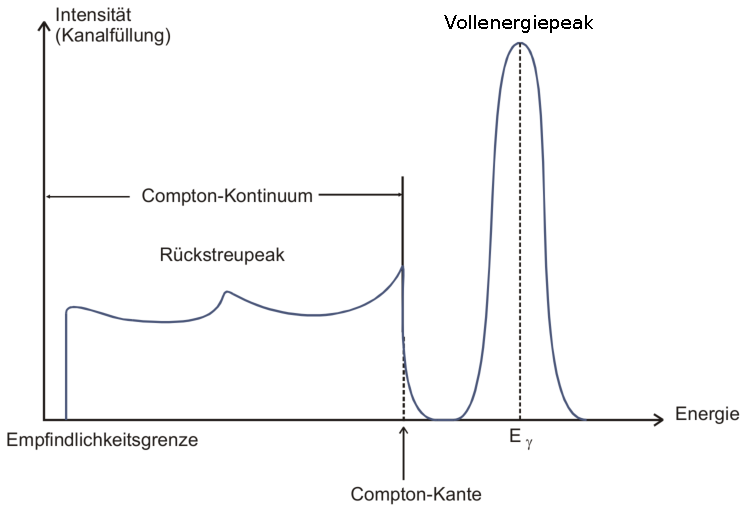
\includegraphics[width=.8\textwidth]{images/typisches-Spektrum.pdf}
	\caption{Schematische Darstellung eines typischen Spektrums einer $\gamma$-Quelle~\cite[23]{anleitung}.}
	\label{fig:typisches-Spektrum}
\end{figure}
